\documentclass[12pt,a4paper]{article}
\usepackage[UTF8]{ctex}
\usepackage{amsmath,amssymb}
\usepackage{xcolor}
\usepackage{hyperref}
\usepackage{geometry}
\usepackage{graphicx}
\geometry{margin=2.5cm}

\title{Variational Quantum Regressor / 变分量子回归器}
\author{QuoNic}
\date{}

\begin{document}
\maketitle

\begin{center}
\textbf{ML / 机器学习} | 难度：高级 | 预计时间：20 分钟
\end{center}

\tableofcontents
\newpage

\section{为什么需要？}

变分量子回归器是经典回归器的量子推广，用于在量子环境中进行回归。

\subsection{经典局限}
\begin{itemize}
  \item 经典回归器在高维数据上训练慢
  \item 对于复杂函数，经典方法效率低
\end{itemize}

\subsection{量子优势}
\begin{itemize}
  \item 变分量子回归器可以利用量子特征映射在高维空间中拟合
  \item 训练速度更快
  \item 可以拟合更复杂的函数
\end{itemize}

\subsection{实际应用}
\begin{itemize}
  \item 函数拟合
  \item 时间序列预测
  \item 数据建模
\end{itemize}

\section{快速上手}

\begin{verbatim}
from quonic.ml import vqr

# 变分量子回归器
x = [0, 1, 2, 3]
y = [0, 1, 4, 9]

result = vqr(x, y, n_layers=2)
print(f'R² score: {result.r2_score}')
\end{verbatim}

\textbf{预期输出}：
\begin{verbatim}
R² score: 0.99
\end{verbatim}

\section{原理详解}

\subsection{电路图}

\begin{center}
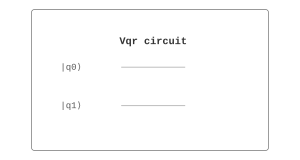
\includegraphics[width=0.6\textwidth]{../../images/vqr_circuit.svg}
\end{center}

\subsection{数学推导}

变分量子回归器：
\begin{equation}
f(x) = \langle 0|U^\dagger(\theta) M U(\theta)|0\rangle
\end{equation}

其中 $U(\theta)$ 是参数化量子电路，$M$ 是测量算子。

\textbf{损失函数}：
\begin{equation}
L(\theta) = \frac{1}{N} \sum_i (f(x_i) - y_i)^2
\end{equation}

\textbf{梯度下降}：
\begin{equation}
\theta_{t+1} = \theta_t - \eta \nabla L(\theta_t)
\end{equation}

\subsection{几何解释}

变分量子回归器在量子态空间中拟合函数。量子特征映射将数据映射到高维空间，使得非线性函数可以用线性模型拟合。

\section{代码详解}

\begin{verbatim}
from quonic.ml import vqr

# vqr(x, y, n_layers, learning_rate)
# x: 自变量
# y: 因变量
# n_layers: 量子电路层数
# learning_rate: 学习率

result = vqr(
    x=[0, 1, 2, 3],
    y=[0, 1, 4, 9],
    n_layers=2,
    learning_rate=0.01
)

# result.r2_score: R² 分数
# result.loss: 损失值
# result.params: 优化后的参数
# result predictions: 预测值
print(f'R² score: {result.r2_score}')
\end{verbatim}

\section{进阶用法}

\subsection{场景 1：不同层数}

\begin{verbatim}
from quonic.ml import vqr

x = [0, 1, 2, 3]
y = [0, 1, 4, 9]

for n in [1, 2, 3]:
    result = vqr(x, y, n_layers=n)
    print(f'n={n}: R²={result.r2_score}')
\end{verbatim}

\subsection{场景 2：不同函数}

\begin{verbatim}
from quonic.ml import vqr
import numpy as np

# 不同函数
x = np.linspace(0, 2*np.pi, 20).tolist()

# 正弦函数
y_sin = np.sin(x).tolist()
result_sin = vqr(x, y_sin, n_layers=3)
print(f'Sin: R²={result_sin.r2_score}')

# 二次函数
y_quad = [xi**2 for xi in x]
result_quad = vqr(x, y_quad, n_layers=3)
print(f'Quadratic: R²={result_quad.r2_score}')
\end{verbatim}

\subsection{场景 3：时间序列预测}

\begin{verbatim}
from quonic.ml import vqr
import numpy as np

# 时间序列预测
t = np.arange(0, 10, 0.5).tolist()
y = np.sin(t).tolist()

result = vqr(t, y, n_layers=3)
print(f'R² score: {result.r2_score}')

# 预测未来值
t_future = np.arange(10, 12, 0.5).tolist()
predictions = result.predict(t_future)
print(f'Predictions: {predictions}')
\end{verbatim}

\section{适用场景}

\subsection{函数拟合}

变分量子回归器可以用于拟合复杂函数。量子特征映射可以表示非线性函数。

\subsection{时间序列预测}

变分量子回归器可以用于时间序列预测。量子特征映射可以捕捉时间序列的长期依赖关系。

\subsection{数据建模}

变分量子回归器可以用于数据建模。量子特征映射可以提取数据的高维特征。

\section{常见问题}

\subsection{变分量子回归器和经典回归器有什么区别？}

变分量子回归器使用量子特征映射，可以在更高维的空间中拟合函数。

\subsection{变分量子回归器的精度如何？}

精度取决于量子电路的深度和数据的质量。

\section{学习路径}

\subsection{前置知识}
\begin{itemize}
  \item 量子神经网络
  \item 参数化量子电路
  \item 量子测量
\end{itemize}

\subsection{继续学习}
\begin{itemize}
  \item 量子分类器
  \item 量子核方法
  \item 量子机器学习
\end{itemize}

\section{完整示例代码}

\subsection{示例 1：基本变分量子回归器}

\begin{verbatim}
from quonic.ml import vqr

x = [0, 1, 2, 3]
y = [0, 1, 4, 9]

result = vqr(x, y, n_layers=2)
print(f'R² score: {result.r2_score}')
\end{verbatim}

\section{下载}

\begin{itemize}
  \item [vqr.py](https://github.com/ChrisLee0721/QuoNic/blob/main/examples/vqr/vqr.py)
\end{itemize}

\end{document}
